\documentclass[10pt]{beamer}
%% beamer template and options 
\mode<presentation>
{
  \usetheme{CambridgeUS}
  \usefonttheme{serif}
  \useoutertheme{default}
}\setbeamertemplate{navigation symbols}{} 



\usepackage[utf8]{inputenc}
\usepackage{xcolor,cancel}
\usepackage{../styles/authordate1-4-beamer}
\usepackage{minted}  %%%%  --shell-escape
\usepackage{pgfplots}
\usepackage{xspace}
\usepackage{amsmath}
\usepackage{wasysym}
\usepackage{tikz}
\usetikzlibrary{automata,fit}
\usetikzlibrary{arrows}
\usetikzlibrary{shapes}
\usetikzlibrary{snakes}
\usetikzlibrary{arrows.meta,intersections}
\tikzstyle{every picture}+=[remember picture]
\usetikzlibrary{decorations.markings}





\title[IDL@BME-BIN] % (optional, use only with long paper titles)
{Introduction to Deep Learning} 
\subtitle{Tools and deep learning of NNet}

\author[A. Allauzen] % (optional, use only with lots of authors)
{Alexandre Allauzen}



\institute[ESPCI/Dauphine/PSL] % (optional, but mostly needed)
{

\includegraphics[height=3em]{../logos/espci_blue.png}\hfill
\raisebox{1.75ex}{
\includegraphics[height=1.5em]{../logos/dauphine.png}}\\
\hfill
\includegraphics[height=3em]{../logos/logomiles_white.pdf}
}




\date{12 and 13/01/20} % (optional)





\DeclareMathOperator*{\argmax}{argmax}
\DeclareMathOperator*{\argmin}{argmin}

\newcommand{\ngram}{\mbox{$n$-gram}\xspace} 



%% important : red + bf 
\def\important#1{{\bf \color{red} #1\/}}


%%% basics : 
\newcommand{\real}{\ensuremath{\mathbb{R}}}
\newcommand{\vct}[1]{\ensuremath{\mathbf{#1}}} % a vector / matrix is in bold
\newcommand{\seq}[1]{\ensuremath{\boldsymbol{#1}}}

\newcommand{\transp}[1]{\ensuremath{{#1}^{t} }} % transposition 
%\newcommand{\scal}[2]{\left\langle #1 , #2 \right\rangle} % scalair
%product
\newcommand{\scal}[2]{#1^t#2} % scalair product
\newcommand{\mydot}[2]{\ensuremath{ \transp{#1} #2}} % dot prod
\newcommand{\norm}[1]{\ensuremath{|| #1 ||}} % l2
\newcommand{\normabs}[1]{\ensuremath{ || #1 ||_{1} }} % l1




% vertical vector 
\newcommand{\vv}[1]{
	\left(
	\begin{array}[c]{c}
		#1 
	\end{array}
	\right)
}
% backeted vertical vector 
\newcommand{\vvb}[1]{
	\left[
	\begin{array}[c]{c}
		#1 
	\end{array}
	\right]
}
% raw vertical vector 
\newcommand{\vvr}[1]{
	\begin{array}[c]{c}
		#1 
	\end{array}
}





% words sequences sentences 
\newcommand{\ws}{{w}} % 
\newcommand{\wseq}{{\mathbf{\ws}}} % 
\newcommand{\length}{{L}} % 
\newcommand{\wsseq}[2]{{\ws_{#1}^{#2}}} % word subsequence
\newcommand{\word}[1]{{\it #1}} % an example
\newcommand{\vocab}{{\mathcal{V}}} % vocab

\newcommand{\asymb}{\ensuremath{a}} % symbol of *one* element of the
                                % alignment sequence
\newcommand{\ssymb}{\ensuremath{s}} % symbol of *one* element of the source
\newcommand{\tsymb}{\ensuremath{t}} % symbol of *one* element of the target


\newcommand{\aseq}{\ensuremath{\mathbf{\asymb}}} % alignment sentence
\newcommand{\sseq}{\ensuremath{\mathbf{\ssymb}}} % source sentence
\newcommand{\tseq}{\ensuremath{\mathbf{\tsymb}}} % target sentence


% misc 
\newcommand{\BigO}[1]{\ensuremath{\operatorname{O}\bigl(#1\bigr)}}
\newcommand{\bos}{\texttt{\textless s\textgreater}} 
\newcommand{\eos}{\texttt{\textless/s\textgreater}} 


% machine learning i/o and parameters ...
% params for model 
\newcommand{\param}{\ensuremath{\theta}} 
\newcommand{\params}{\ensuremath{\boldsymbol{\theta}}}
\newcommand{\nfeats}{\ensuremath{D}} % 

\newcommand{\x}{\ensuremath{\seq{x}}} % 
\newcommand{\X}{\ensuremath{\seq{X}}} % 
\newcommand{\y}{\ensuremath{\seq{y}}} % 
\newcommand{\z}{\ensuremath{\seq{z}}} % 
\newcommand{\w}{\ensuremath{\seq{w}}} % 
\newcommand{\pa}{\ensuremath{\seq{a}}} % 
\newcommand{\pb}{\ensuremath{\seq{b}}} % 

\newcommand{\W}{\seq{W}}
\newcommand{\V}{\seq{V}}
\newcommand{\pgrad}[1]{\nabla_{#1}}
\newcommand{\vgrad}[2]{\ensuremath{\nabla_{#1} #2}}

%%%%%%% data and loss
\newcommand{\nsamples}{\ensuremath{N}}
\newcommand{\ploss}{\ensuremath{l}} % for one datapoint
\newcommand{\class}{\ensuremath{{c}}} %
\newcommand{\rvclass}{\ensuremath{{C}}} %  the class as a RV 
\newcommand{\sid}[1]{\ensuremath{_{(#1)}}} % sample id
\newcommand{\tid}[1]{_{(#1)}} % time index for parameters
\newcommand{\exi}{\ensuremath{\x\sid{i}}} % 
\newcommand{\classi}{\ensuremath{\class\sid{i}}} % 
\newcommand{\nclasses}{\ensuremath{C}} % 
\newcommand{\yi}{y\sid{i}}  % prediction for sample i 

\newcommand{\dataset}{\ensuremath{\mathcal{D}}} % training data
\newcommand{\datax}{\ensuremath{\mathcal{X}}} % training data, x part
\newcommand{\datay}{\ensuremath{\tilde{\mathcal{Y}}}} % training data y part  
\newcommand{\datac}{\ensuremath{\tilde{\mathcal{C}}}} % training data c part (classes)
\newcommand{\ty}{\ensuremath{\tilde{y}}} % the supervised answer
\newcommand{\fullloss}{\ensuremath{\mathcal{L}(\params;\dataset)}}

%%% 
\newcommand{\nlaw}{\mathcal{N}}
\newcommand{\bern}{\ensuremath{\pi}}



%%%%%%%%%%%%%%%%%%%%%%%%%%%%%%%%%%%%%%%%%%%%%%%%%%%%%%%%%%%%
% a vector as a grid 
% 1: x 
% 2: y
% 3: the number of cells 
% The template :
% \node[rectangle,rounded corners,  draw, fill=red!20, text width=0.3*\textwidth, minimum height=6ex]  (label) at (0,0) {Hello} ;
\newcommand{\xvector}[3]{%
  \draw[step=.25] (#1-0.001,#2) grid (#1+0.25,#2+#3*0.25 );%
}

% notations 
% a layer l 
% input x^{(l)}
% output y^{(l)}
%  y^{(l)} = f^{(l)}( W^{(l)} input)
% note that 
% y_i = W_i,: x
% W_ij : x_j -> y_i  
% k is for the class
% l for the layer 


%%%%%%% to define layers math notations 
\newcommand{\inp}{\ensuremath{\x}}
\newcommand{\outp}{\ensuremath{\seq{y}}}
\newcommand{\lid}[1]{\ensuremath{^{(#1)}}}

%%%%%%% data and loss
\newcommand{\dlta}{\ensuremath{\delta}} % gradient component of pre-activation
\newcommand{\vdlta}{\ensuremath{\seq{\delta}}} % gradient vector of pre-activation

\colorlet{darkgreen}{green!50!black}


%% draw one layer 
\newcommand{\layer}{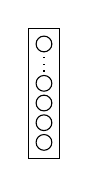
\begin{tikzpicture}[baseline=0.5ex]%
    \foreach \y in {0.25,0.5,...,1}{ 
      \draw (0,\y) circle  (0.1);%
    }
    \draw[dotted] (0.0, 1.15) -- (0.0,1.35); 
    \draw (0,1.5) circle (0.1);
    \draw (-0.2,0.05) rectangle (0.2,1.7);
\end{tikzpicture}}

%% draw connection
\newcommand{\connection}{\begin{tikzpicture}[baseline=0.5ex]%
    \draw[->] (0,0.85) -- (1.0,0.85);
\end{tikzpicture}}
%% dotted connection
\newcommand{\dotted}{\begin{tikzpicture}[baseline=0.5ex]%
    \draw[dotted,thick] (0,0.85) -- (0.5,0.85);%
\end{tikzpicture}}

\newcommand{\raiseW}{2ex}
% for computational graph
\newcommand{\vnode}{\node}
\newcommand{\funnode}{\node[minimum size=1.5,rectangle,draw=green,fill=green!20]}
\newcommand{\inlinefnode}[1]{\raisebox{-5pt}{\tikz{\funnode {#1}}}}



\newcommand{\justunder}{0.5cm}
\newcommand{\largeurUn}{0.8}
\newcommand{\largeurDeux}{0.7}
\setbeamercolor{postit}{fg=black,bg=red!30}
\setbeamercolor{mygreen}{fg=black,bg=green!20}
\setbeamercolor{myred}{fg=black,bg=red!20}
\setbeamercolor{darkpostit}{fg=black,bg=red!64}
\setbeamercolor{text}{fg=black,bg=red!10}


%%%%%%%%%% NNet for NLP
%% draw one layer  
\newcommand{\wemb}{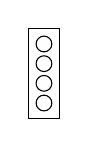
\begin{tikzpicture}[baseline=0.5ex]%
    \foreach \y in {0.25,0.5,...,1}{ 
      \draw (0,\y) circle  (0.1);%
    }
    \draw (-0.2,0.05) rectangle (0.2,1.2);
\end{tikzpicture}}

\newcommand{\worddim}{\ensuremath{K}} % dimension of the word embeddings
\newcommand{\wvector}{\ensuremath{\vct{v}}} % word vector
\newcommand{\wmatrix}{\ensuremath{\vct{R}}} % word matrix
\newcommand{\dvector}{\ensuremath{\vct{d}}} % document vector



%%%%%%%%% macro et redefinition 
\AtBeginSection[]
{
  \begin{frame}<beamer>
    \frametitle{Outline}
    \tableofcontents[currentsection]
  \end{frame}
}


\begin{document}
\tikzset{->-/.style={decoration={
  markings,
  mark=at position .5 with {\arrow{>}}},postaction={decorate}}}

\begin{frame}
  \titlepage
\end{frame}

\begin{frame}<beamer>
  \frametitle{Outline}
  \tableofcontents
\end{frame}
 



\section{Deep Learning: introduction}
\begin{frame}
  \frametitle{Two layers fully connected: a linear separation}
  \begin{center}
    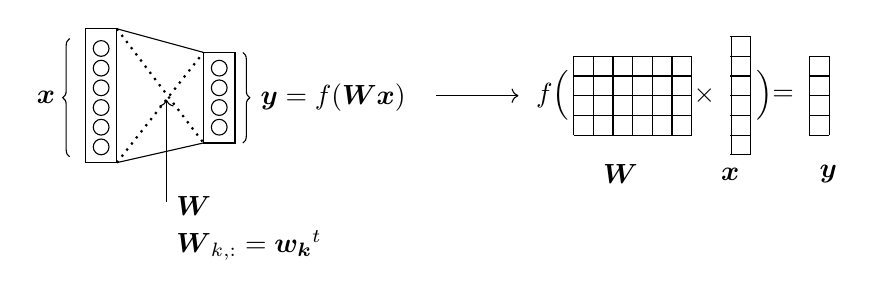
\begin{tikzpicture}
      \begin{scope}
        % input
        \node (nx) at (-0.7,0.625){$\x$}; %
        \foreach \y in {0,0.25,...,1.25}{ 
          \draw (0,\y) circle  (0.1cm);%
        }
        \draw (-0.2,-0.2) rectangle (0.2,1.5);
        \draw[snake=brace] (-0.4,-0.125) -- (-0.4,1.375); 
        % output
        \foreach \y in {0.25,0.5,...,1}{ 
          \draw (1.5,\y) circle  (0.1cm);%
        }
        \draw (1.3,0.05) rectangle (1.7,1.2);
        \draw (0.2,-0.2) -- (1.3,0.05); 
        \draw (0.2,1.5) -- (1.3,1.2);
        \draw[dotted, thick] (0.2,1.5) -- (1.3,0.05);
        \draw[dotted,thick] (0.2,-0.2) -- (1.3,1.2); 
        \draw[snake=brace] ( 1.8, 1.2) --(1.8, 0.05) ; 
        \node[anchor=west] (ny) at (1.9,0.625){$\seq{y}=f(\W \x)$}; %
        \node[anchor=west] (nW) at (0.83,-0.75){$\W$};%
        \node[anchor=west] (nW) at (0.83,-1.25) {$\W_{k,:}=\seq{w_k}^t$}; %
        \draw[->]  (0.83,-0.7) -- (0.83,0.6);%
      \end{scope}
      %%%%%%%%%%%%%%%%%%%%%%%%%%%%%%%%%%%%%%%%%% 
      %% matrix view 
      %%%%%%%%%%%%%%%%%%%%%%%%%%%%%%%%%%%%%%%%%% 
      \only<2->{
        \begin{scope}[xshift=6cm,yshift=0.15cm]
          
          \draw[->] (-1.75,0.5) -- (-0.7,0.5);
          \draw[step=.25] (0,-0) grid (1.5, 1);%
          \draw[step=.25] (1.99,-0.25) grid (2.25, 1.25 );%
          \draw[step=.25] (2.99,-0) grid (3.25, 1 );%
          % oper
          \node[anchor=west] (times) at (1.4, 0.5) {$\times$};
          \node[anchor=west] (equals) at (2.4, 0.5) {$=$};
          % names
          \node[anchor=west] (f) at (-0.6, 0.5) {$f\Big($};
          \node[anchor=west] (fe) at (2.2, 0.5) {$\Big)$};
          \node[anchor=west] (W) at (0.25, -0.5) {$\seq{W}$};
          \node[anchor=west] (x) at (1.75, -0.5) {$\seq{x}$};
          \node[anchor=west] (x) at (3, -0.5) {$\seq{y}$};
        \end{scope}
      }
    \end{tikzpicture}
  \end{center}
  \pause\pause
  {
    \begin{columns}
      \column{0.5\textwidth}
      Activation $f$:
      \begin{itemize}
      \item $f$ is usually a non-linear function
      \item $f$ is a component wise function
      \item tanh, sigmoid, relu, ...
      \end{itemize}
      \column{0.5\textwidth}
      Dimensions: 
      \begin{itemize}
      \item $\x: \nfeats \times 1 $
      \item $\seq{W}: \nclasses \times \nfeats $
      \item $\seq{y}: (\nclasses \times \xcancel{ \nfeats) \times (  \nfeats }
        \times 1 ) =\nclasses \times 1 $
      \end{itemize}
    \end{columns}
    \textit{e.g} the softmax function:
    $$      
    y_k = P(c=k|\x) = \frac{e^{\scal{\seq{w_k}}{\x}} }{\sum_{k'}e^{\scal{\seq{w_{k'}}}{\x}}}
    = \frac{e^{\W_{k,:}\x}}{\sum_{k'} e^{\W_{k',:}\x}}
    $$   
  }
\end{frame}


\begin{frame}{From linear to non-linear case}
  \begin{columns}
    \begin{column}{0.7\textwidth}
      \begin{center}
        \begin{tabular}[h]{lclclr}
          \color{red}\inp\lid{1} & & \inp\lid{2}  && \\
          \color{red}\layer &\connection &\layer &\connection &\layer \\[-2ex]
          & \raisebox{\raiseW}{\W\lid{1}} &\outp\lid{1}   &\raisebox{\raiseW}{\W\lid{2}} &\color{red}\outp\lid{2}: output 
        \end{tabular}
      \end{center}
     \end{column}
    \begin{column}{0.3\textwidth}
      $$\params=(\W\lid{1},\W\lid{2})$$
      Trained by back-propagation of the gradient
    \end{column}
  \end{columns}
  \begin{block}{Universal approximation theorem}

    \begin{quote}
      a feed-forward network with a single hidden layer containing a
      finite number of neurons can approximate continuous functions on
      compact subsets of $\real^n$, under mild assumptions on the
      activation function. (...)
    \end{quote}
    \begin{flushright}
      \cite{Cybenko89Approximation}
    \end{flushright}
    However, it does not touch upon the algorithmic learnability of those parameters.
  \end{block}
\end{frame}


\begin{frame}{Overfitting}
  \framesubtitle{The danger of the over-parametrization}
  \begin{center}
    \includegraphics[width=0.5\textwidth]{../figs/overfitting-1}\hfill
    \includegraphics[width=0.4\textwidth]{../figs/overfitting-2}
  \end{center}
  {\small Source: Wikipedia}
\end{frame}



\begin{frame}{Multi-layer neural network (feed-forward)}
  \begin{block}{One layer, indexed by $l$}
    \begin{columns}
      \begin{column}{0.3\textwidth}
        \begin{tabular}[h]{lcl}
          \inp\lid{l} & & \\
          \layer &\connection &\layer\\[-2ex]
          & \raisebox{\raiseW}{\W\lid{l}} &\outp\lid{l} 
        \end{tabular} 
      \end{column}
      \begin{column}{0.7\textwidth}
        \begin{itemize}
        \item \inp\lid{l}: input of the layer $l$
        \item \outp\lid{l} =  $f$\lid{l}(\W\lid{l} \inp\lid{l})
        \item stacking layers:  \outp\lid{l} $=$ \inp\lid{l+1} 
        \item \inp\lid{1}  = a data example
        \end{itemize}
      \end{column}
    \end{columns}
  \end{block}
  
  \vspace{-2ex}
  \begin{center}
    \begin{tabular}[h]{lclclclclcl}
      \color{red}\inp\lid{1} & & \inp\lid{2}  && \inp\lid{3} & &\inp\lid{L} \\
      \color{red}\layer &\connection &\layer &\connection &\layer &\dotted &\layer &\connection &\color{red}\layer \\[-2ex]
      & \raisebox{\raiseW}{\W\lid{1}} &\outp\lid{1}   &\raisebox{\raiseW}{\W\lid{2}} &\outp\lid{2}  &&\outp\lid{L-1}&\raisebox{\raiseW}{\W\lid{L}} &\color{red}\outp\lid{L}: output 
    \end{tabular}
  \end{center}
\end{frame}






%%%%%%%%%%%%%%%%%%%%%%%%%%%%%%%%%%%%%%%%%%%%%%%%%%%%%%%%%%%%%%%%%%%%%%
\section{Vanishing gradient}
%%%%%%%%%%%%%%%%%%%%%%%%%%%%%%%%%%%%%%%%%%%%%%%%%%%%%%%%%%
%
% WARNING : use common_nnet.tex
%
%%%%%%%%%%%%%%%%%%%%%%%%%%%%%%%%%%%%%%%%%%%%%%%%%%%%%%%%%%


%the different layers in our deep network are learning at vastly different speeds. In particular, when later layers in the network are learning well, early layers often get stuck during training, learning almost nothing at all.
%there's an intrinsic instability associated to learning by gradient descent in deep, many-layer neural networks. This instability tends to result in either the early or the later layers getting stuck during training
\begin{frame}{Experimental observations (MNIST task) - 1}
  \begin{block}{The MNIST database}
    \includegraphics[width=0.6\textwidth]{../figs/mnist}
  \end{block}
  \begin{block}{Comparison of different depth for feed-forward architecture}
     \begin{center}
       \resizebox{0.8\columnwidth}{!}{
         \begin{tabular}[h]{lclclclclcl}
          \color{red}\inp\lid{1} & & \inp\lid{2}  && \inp\lid{3} & &\inp\lid{L} \\
          \color{red}\layer &\connection &\layer &\connection &\layer &\dotted &\layer &\connection &\color{red}\layer \\[-2ex]
          & \raisebox{\raiseW}{\W\lid{1}} &\outp\lid{1}   &\raisebox{\raiseW}{\W\lid{2}} &\outp\lid{2}  &&\outp\lid{L-1}&\raisebox{\raiseW}{\W\lid{L}} &\color{red}\outp\lid{L}: output 
        \end{tabular}
      }
      \begin{itemize}
      \item Hidden layers have a sigmoid activation function.
      \item The output layer is a softmax.
      \end{itemize}
  \end{center}
  \end{block}
\end{frame}

\begin{frame}{Experimental observations (MNIST task) - 2}
  \begin{block}{Varying the depth}
    \begin{itemize}
    \item Without hidden layer:  $\approx 88\%$ accuracy
    \item 1 hidden layer (30): $\approx 96.5\%$ accuracy
    \item 2 hidden layers (30): $\approx 96.9\%$ accuracy
    \item 3 hidden layers (30): $\approx 96.5\%$ accuracy
    \item 4 hidden layers (30): $\approx 96.5\%$ accuracy
    \end{itemize}
  \end{block}\pause
  \begin{columns}
    \begin{column}{0.5\textwidth}
      \includegraphics[width=1\textwidth]{../figs/training_speed_4_layers}
    \end{column}
    \begin{column}{0.5\textwidth}
      \scriptsize (From \url{http://neuralnetworksanddeeplearning.com/chap5.html})
    \end{column}
  \end{columns}
\end{frame}


\begin{frame}{Intuitive explanation}
  Let consider the simplest deep neural network, with just a single neuron in each layer.
  \begin{center}
    \includegraphics[width=0.7\textwidth]{../figs/oneUnitNet}
  \end{center}
  $w_i, b_i$ are resp. the weight and bias of neuron $i$ and $C$ some cost function. 
  \begin{block}{Compute the gradient of $C$ \textit{w.r.t} the bias $b_1$}
    \begin{align}
      \frac{\partial C }{\partial b_1} &=       \frac{\partial C}{\partial y_4}      \times
      \frac{\partial y_4}{\partial a_4}   \times \frac{\partial a_4}{\partial y_3} \times
      \frac{\partial y_3}{\partial a_3}   \times \frac{\partial a_3}{\partial y_2} \times
      \frac{\partial y_2}{\partial a_2}   \times \frac{\partial a_2}{\partial y_1} \times
      \frac{\partial y_1}{\partial a_1}   \times \frac{\partial a_1}{\partial b_1} \\
      &=       \frac{\partial C}{\partial y_4}      \times
      \sigma'(a_4) \times w_4 \times
      \sigma'(a_3) \times w_3 \times
      \sigma'(a_2) \times w_2 \times
      \sigma'(a_1) 
    \end{align}
  \end{block}
\end{frame}

\begin{frame}{Intuitive explanation - 2}
  \begin{block}{The derivative of the activation function: $\sigma'$}
    \begin{columns}
      \begin{column}{0.5\textwidth}
%%%%%%% logistic
          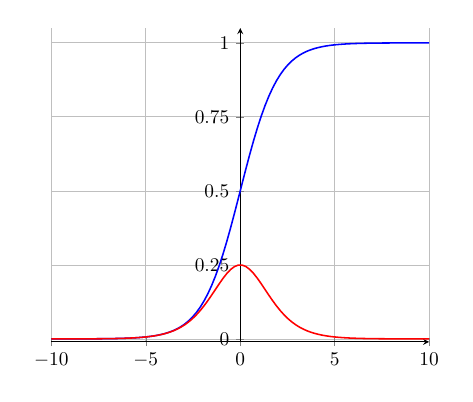
\begin{tikzpicture}[scale=0.7]
            \begin{axis}%
              [ %%%%%%%%%%%%%%%%%
              grid=major, %
              xmin=-10, % 
              xmax=10, % 
              axis x line=bottom, % 
              ytick={0,.25,.5,.75,1.0}, %
              ymax=1.05, % 
              ymin = -0.01, %
              axis y line=middle, % 
              every  axis y label/.style={at={(current axis.north
                  west)},above=2mm} ]% 
              \addplot%
              [ blue,thick,%
              mark=none, samples=100, domain=-10:10, ]
              (x,{ (1/(1+exp(-x))) });
              \addplot%
              [ red,thick,%
              mark=none, samples=100, domain=-10:10, ]
              (x,{ (1/(1+exp(-x)))*(1-(1/(1+exp(-x)))) });
            \end{axis}
          \end{tikzpicture}
      \end{column}
      \begin{column}{0.5\textwidth}
        $$
        \sigma'(x) = \sigma(x)(1-\sigma(x))
        $$
        But weights are initialize around $0$. 
      \end{column}
    \end{columns}
  \end{block}
  \important{The different layers in our deep network are learning at vastly different speeds:}
  \begin{itemize}
  \item when later layers in the network are
    learning well,
  \item early layers often get stuck during training,
    learning almost nothing at all.
\end{itemize}
\end{frame}

\begin{frame}{A first Solution}
  \begin{block}{Change the activation function (Rectified Linear Unit or
      ReLU)}
    \begin{columns}
      %%%%%%%%% relu
      \begin{column}{0.4\textwidth}
        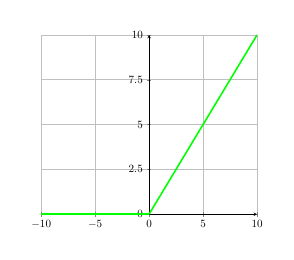
\begin{tikzpicture}[scale=0.4]
          \begin{axis}%
            [ %%%%%%%%%%%%%%%%%
            grid=major, %
            xmin=-10, % 
            xmax=10, % 
            axis x line=bottom, % 
            ytick={0,2.5,5,7.5,10}, %
            ymax=10, % 
            ymin = -0.01, %
            axis y line=middle, % 
            every  axis y label/.style={at={(current axis.north
                west)},above=2mm} ]%
            \addplot%
            [ green,line width=0.5mm,%
            mark=none, samples=100, domain=0:-10, ]
            (x,{0.00});
            \addplot%
            [ green,line width=0.5mm,%
            mark=none, samples=100, domain=0:10, ]
            (x,x);
          \end{axis}
        \end{tikzpicture}
      \end{column}
      \begin{column}{0.6\textwidth}
        \begin{itemize}
        \item Avoid the vanishing gradient
        \item  Some units can "die''
        \end{itemize}
        See~\cite{Glorot11Rectifier} for more details
      \end{column}
    \end{columns}
  \end{block}
  \begin{block}{Variants}
    \begin{itemize}
    \item Leaky ReLU~\cite{Maas13lrelu}
    \item Soft-plus $log(1+e^x)$
    \end{itemize}
    And many more, see \url{https://pytorch.org/docs/stable/nn.html}
  \end{block}
  \begin{block}{More details}
    See~\cite{Hochreiter01Gradient,Glorot10Understanding,Lecun12Efficient} 
  \end{block}
\end{frame}


% \begin{frame}{A question}
%   Why adding a layer can lower the performance ? \pause
%   \begin{itemize}
%   \item Overfitting ? and what about the identity
%   \item Vanishing gradient ? and with the \textit{Relu} ? 
%   \end{itemize} \pause
%   \begin{block}{Residual block}
%     \begin{columns}
%     \column{0.5\textwidth}
%     From~\cite{He16Residual}
%     \begin{itemize}
%     \item Add a skip connection
%     \item The model learn the "residual"
%       $$
%       \y = \mathcal{F}(\x) = \x + \mathcal{R}(\x)
%       $$
%     \end{itemize}
%       \column{0.5\textwidth}
%       \begin{center}
%         \includegraphics[width=\textwidth]{../figs/residual}
%       \end{center}
%     \end{columns}
%     A simple version of highway networks~\cite{Srivastava15Highway}
%   \end{block}
% \end{frame}


% \begin{frame}{Residual block}
%   \begin{block}{Forward}
%     \begin{align*}
%       \y &= \mathcal{F}(\x) = \x + \mathcal{R}(\x), \textrm{ or }\\
%       \y &= \W_{s} \x + \mathcal{R}(\x), \textrm{ to adapt the dimension}
%     \end{align*}
%   \end{block}
%   \begin{block}{Backward}
%     Assume a residual block for the layer $l$ in the network. Training requires:
%     \begin{itemize}
%     \item $\frac{\partial l }{\partial\W\lid{l}}$ for the update of the layer
%     \item $\frac{\partial l }{\partial\x\lid{l}}$ for the backpropagation
%     \end{itemize}
%     \begin{align*}
%       \frac{\partial l }{\partial\x\lid{l}} &=       \frac{\partial l }{\partial\y\lid{l}} \times  \frac{\partial\y\lid{l}}{\partial\x\lid{l}}\\
%                                             &= \frac{\partial l }{\partial\y\lid{l}} \times  (1+\frac{\partial\mathcal{R}(\x\lid{l})}{\partial\x\lid{l}})
%     \end{align*}
%   \end{block}
% \end{frame}



\section{Regularization}
% Regularization  + Dropout 

\begin{frame}{Regularization $l^2$ or gaussian prior or weight decay}
  The basic way: 
  $$
  \fullloss = \sum_{i=1}^{\nsamples} \ploss(\params,\exi,\classi)  {\color{red}+ \frac{\lambda}{2} || \params||^2}
  $$
  \begin{itemize}
  \item The second term is the {\color{red}regularization term}. 
  \item Each parameter has a gaussian prior : $
    \mathcal{N}(0,1/\lambda)$.
  \item $\lambda$ is a hyperparameter. 
  \item  The update has the form:
    $$
    \params = (1+\eta_t\lambda) \params - \eta_t \pgrad{\params} 
    $$
  \end{itemize}
\end{frame}

\begin{frame}{Dropout}
  \framesubtitle{A new regularization
    scheme~\cite{Srivastava14Multimodal}}
  \begin{columns}
    %%%%%%%%%%%%%%%%%%%%%%
    \begin{column}{0.5\textwidth}
      \begin{center}
        \includegraphics[width=1\textwidth]{../figs/dropout2}
      \end{center}
    \end{column}
    %%%%%%%%%%%%%%%%%%%%%%
    \begin{column}{0.5\textwidth}
      \begin{itemize}
      \item  For each training example:  randomly turn-off the neurons
        of hidden units (with $p=0.5$)
      \item  At test time, use each neuron scaled down by $p$
      \end{itemize}
    \end{column}
  \end{columns}
  %%%%%%%%%%%%%%%%%%%%%%
  \begin{itemize}
  \item  Dropout serves to separate effects from strongly correlated
    features and 
  \item prevents co-adaptation between units
  \item It can be seen as averaging different models that share parameters.
  \item It acts as a powerful regularization scheme. 
  \end{itemize}
\end{frame}
% Dropout is known to work well, although not always:

%     In vision tasks, input features are commonly dense, while in our
%     task input features are sparse and labels are noisy. In the dense
%     setting, dropout serves to separate effects from strongly
%     correlated features, resulting in a more robust classifier. But in
%     our sparse, noisy setting adding in dropout appears to simply
%     reduce the amount of data available for learning.


\begin{frame}{Dropout - implementation}
  The layer should keep: 
  \begin{itemize}
  \item $\W\lid{l}$: the parameters
  \item $f\lid{l}$: its activation function
  \item $\inp\lid{l}$: its input
  \item $\seq{a}\lid{l}$: its pre-activation associated to the input
  \item $\vdlta\lid{l}$: for the update and the back-propagation to the layer $l-1$
  \item {\color{red} $\seq{m}\lid{l}$: the dropout mask}, to be applied
    on $\inp\lid{l}$ 
  \end{itemize}
  \begin{block}{Forward pass}
        For $l=1$ to $(L-1)$
    \begin{itemize}
    \item Compute $\outp\lid{l}=f\lid{l}(\W\lid{l}\inp\lid{l})$
    \item $\inp\lid{l+1} =\outp\lid{l} = \outp\lid{l} \circ \seq{m}\lid{l}$
    \end{itemize}
    $\outp\lid{L}=f\lid{L}(\W\lid{L}\inp\lid{L})$
  \end{block}
\end{frame}

%%%%%%%%%%%%%%%%%%%%%%%%%%%%%%%%%%%%%%%%%%%%%%%%%%%%%%%%%%%%%%%%%%%%%%
\section{Pytorch: computation graph}
\begin{frame}
  \frametitle{Some useful libraries}
  \begin{block}{Theano}
    Written in python by the LISA (Y. Bengio and I. Goodfellow),
    low-level API.
  \end{block}
  \begin{block}{TensorFlow and Keras}
    The Google library with python API + high level API
  \end{block}
  \begin{block}{pyTorch}
    The Facebook library with python API 
  \end{block}
  \begin{block}{And others}
    Caffe, MXNet, CNTK, Chainer, ...
  \end{block}
  \begin{itemize}
  \item CPU/GPU
  \item Automatic differentiation based on computational graph
  \end{itemize}
\end{frame}


\begin{frame}{Computation graph}
  A convenient way to represent  a  complex mathematical expressions: 
  \begin{itemize}
  \item  each node is an operation or a variable
  \item an operation has some inputs / outputs made of variables
  \end{itemize}
  \begin{block}{Example 1 : A single  layer network}
    \begin{columns}
      \begin{column}{0.5\textwidth}
        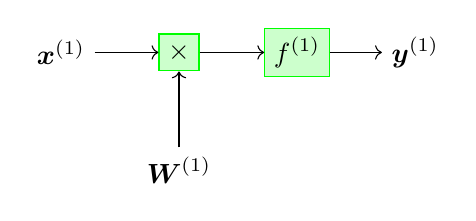
\begin{tikzpicture}
          \vnode (x1) at (0,0) {$\x\lid{1}$}; % 
          \vnode (W1) at  (1.5,-1.5) {$\W\lid{1}$};  % 
          \funnode (dot1) at (1.5,0) {$\times$};%
          \funnode (f1) at (3,0) {$f\lid{1}$}; 
          \vnode (y1) at (4.5,0)  {$\outp\lid{1}$}; 
          \draw[->] (x1) -- (dot1); 
          \draw[->] (dot1) -- (f1); 
          \draw[->] (W1) -- (dot1); 
          \draw[->] (f1) -- (y1);
        \end{tikzpicture}
      \end{column}
      \begin{column}{0.5\textwidth}
        \begin{itemize}
        \item Setting $\inp\lid{1}$ and $\W\lid{1}$
        \item Forward pass $\rightarrow \outp\lid{1}$
        $$ 
        \outp\lid{1} = f\lid{1}(\W\lid{1}\inp\lid{1})
        $$
        \end{itemize}
      \end{column}
    \end{columns}
  \end{block}
  \begin{block}{Remark}
    Some toolkit refers to variable as node, and function as edge. 
  \end{block}
\end{frame}


\begin{frame}{Building a computation graph}
  \begin{quote}
    Variables (eq. Tensors) flow through a D.A.G
  \end{quote}
  \begin{block}{A variable is a  \textit{Tensor}}
    A \textit{Tensor} stores: 
    \begin{itemize}
    \item the values (as \textit{numpy.array}); 
    \item a link to its creator;
    \item (optionally) the gradient values (as a \textit{numpy.array} of same size);
    \end{itemize}
    The creator is a function or tensor operation 
  \end{block}
  \begin{block}{Function}
    A tensor operation that takes:
    \begin{itemize}
    \item several (or zero) input tensors,
    \item and output one new tensor as a result. 
    \end{itemize}
  \end{block}
\end{frame}


\begin{frame}{Ex: the logistic regression model}
  \framesubtitle{The computation graph}
  \begin{center}
    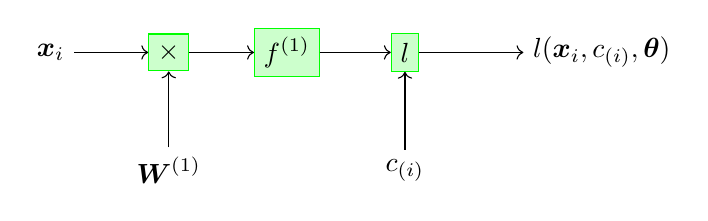
\begin{tikzpicture}
      \vnode (x2) at (0,0) {$\x_i$}; % 
      \vnode (W2) at  (1.5,-1.5) {$\W\lid{1}$};  % 
      \funnode (dot2) at (1.5,0) {$\times$};%
      \funnode (f2) at (3,0) {$f\lid{1}$}; 
      \funnode (loss) at (4.5,0) {$\ploss$}; 
      \vnode (label) at  (4.5,-1.5) {$\classi$};  % 
      \vnode (outloss) at  (7,0) {$\ploss(\x_i,\classi,\params)$};  % 
      \draw[->] (x2) -- (dot2); 
      \draw[->] (dot2) -- (f2); 
      \draw[->] (W2) -- (dot2); 
      \draw[->] (f2) -- (loss);
      \draw[->] (label) -- (loss);
      \draw[->] (loss) -- (outloss);
    \end{tikzpicture}
  \end{center}
  \begin{itemize}
  \item $f\lid{1}$ is the sigmoid ($\sigma$) function
  \item the loss is the binary log-loss (a.k.a binary cross
    entropy):
    $$
    \ploss(\inp, \class, \params=\W)  %
    = \classi \log y + (1-\classi) \log (1-y),
    $$
  \item with $y$, a scalar, the output of $f\lid{1}$.
  \end{itemize}
\end{frame}

\begin{frame}[fragile]{Ex: the logistic regression model}
  \framesubtitle{In numpy \textit{vs} pytorch}
  \begin{center}
    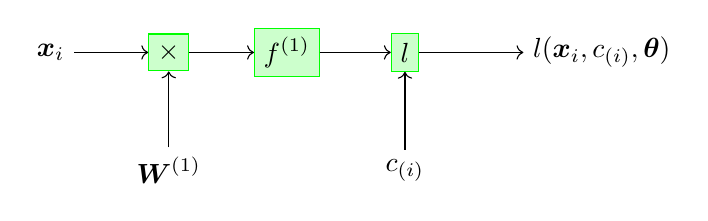
\begin{tikzpicture}{scale=0.9}
      \vnode (x2) at (0,0) {$\x_i$}; % 
      \vnode (W2) at  (1.5,-1.5) {$\W\lid{1}$};  % 
      \funnode (dot2) at (1.5,0) {$\times$};%
      \funnode (f2) at (3,0) {$f\lid{1}$}; 
      \funnode (loss) at (4.5,0) {$\ploss$}; 
      \vnode (label) at  (4.5,-1.5) {$\classi$};  % 
      \vnode (outloss) at  (7,0) {$\ploss(\x_i,\classi,\params)$};  % 
      \draw[->] (x2) -- (dot2); 
      \draw[->] (dot2) -- (f2); 
      \draw[->] (W2) -- (dot2); 
      \draw[->] (f2) -- (loss);
      \draw[->] (label) -- (loss);
      \draw[->] (loss) -- (outloss);
    \end{tikzpicture}
  \end{center}
  \begin{columns}
    \small 
    \column{0.4\textwidth}
  \begin{minted}{python}
    import numpy as np
    # explicite bias 
    W = np.random.randn(1,D+1) 
    # inference
    # x the input:  np.array
    a = W@x 
    y = 1/(1+np.exp(-a))
    # a and y are np.array
    # loss: c (target) np.array~~~
    l = -c*np.log(y)
        - (1-c)*np.log(1-y) 
  \end{minted}
  \column{0.6\textwidth}
  \begin{minted}{python}
    import torch as th
    # explicite bias 
    W = th.randn(1,D+1,requires_grad=True)
    # inference
    # x is a th.Tensor 
    a = W@x # or W.matmul(x)
    y = 1/(1+th.exp(-a)) 
    # a and y are th.Tensor
    # loss: c (target), a th.Tensor
    l = -c*th.log(y)
        - (1-c)*th.log(1-y) 
  \end{minted}
\end{columns}
\end{frame}





 
\begin{frame}{Ex: the logistic regression model}
  \framesubtitle{Compute the gradient}
       \begin{center}
          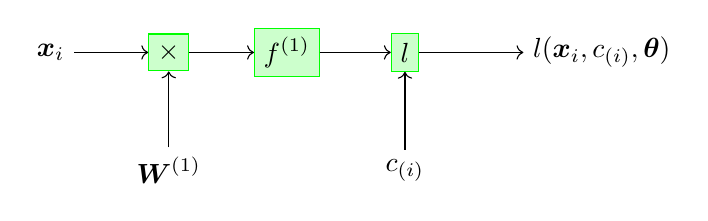
\begin{tikzpicture}{scale=0.9}
          \vnode (x2) at (0,0) {$\x_i$}; % 
          \vnode (W2) at  (1.5,-1.5) {$\W\lid{1}$};  % 
          \funnode (dot2) at (1.5,0) {$\times$};%
          \funnode (f2) at (3,0) {$f\lid{1}$}; 
          \funnode (loss) at (4.5,0) {$\ploss$}; 
          \vnode (label) at  (4.5,-1.5) {$\classi$};  % 
          \vnode (outloss) at  (7,0) {$\ploss(\x_i,\classi,\params)$};  % 
          \draw[->] (x2) -- (dot2); 
          \draw[->] (dot2) -- (f2); 
          \draw[->] (W2) -- (dot2); 
          \draw[->] (f2) -- (loss);
          \draw[->] (label) -- (loss);
          \draw[->] (loss) -- (outloss);
        \end{tikzpicture}
        \end{center}
        The goal :
        $$\frac{\partial \ploss}{\partial \W\lid{1}} = \frac{\partial
          \ploss}{\partial \outp}  \frac{\partial \outp}{\partial
          \seq{a}} \frac{\partial \seq{a}}{\partial \W\lid{1}}  $$
        Gradient computation: 
        $$ \inlinefnode{\ploss} \rightarrow
        % 
        {\color{red} \frac{\partial \ploss}{\partial \outp}} \rightarrow
        % 
        \inlinefnode{$f$}  \rightarrow
        %
        \frac{\partial \ploss}{\partial \outp}  {\color{red} \frac{\partial \outp}{\partial
          \seq{a}}} \rightarrow
        %
        \inlinefnode{$\times$}  \rightarrow
        %
        \frac{\partial
         \ploss}{\partial \outp}  \frac{\partial \outp}{\partial
        \seq{a}}  {\color{red} \frac{\partial \seq{a}}{\partial \W\lid{1}} }
      $$
      \begin{center}
%        In pytorch : \textit{l.backward()} ! 
      \end{center}
\end{frame}


\begin{frame}{The computation graph in both directions}
  % Use funnode and vnode see common_nnet.tex 
  %
  \begin{center}
    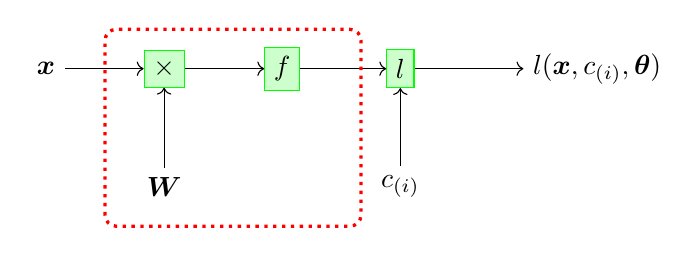
\begin{tikzpicture}
      \vnode (x2) at (0,0) {$\x$}; % x
      \vnode (W2) at (1.5,-1.5) {$\W$}; % W
      \funnode (dot2) at (1.5,0) {$\times$};% x
      \funnode (f2) at (3,0) {$f$};
      \funnode (loss) at (4.5,0) {$\ploss$};  % loss 
      \vnode (label) at (4.5,-1.5) {$\classi$}; % the class 
      \vnode (outloss) at (7,0) {$\ploss(\x,\classi,\params)$}; % out value
      %%%% graph links 
      \draw[->] (x2) -- (dot2);
      \draw[->] (dot2) -- (f2);
      \draw[->] (W2) -- (dot2);
      \draw[->] (f2) -- (loss);
      \draw[->] (label) -- (loss);
      \draw[->] (loss) -- (outloss);
      %%%%% draw a box around the NNet
      \draw[red,dotted,very thick,rounded corners] (0.75,-2) rectangle (4,0.5);
    \end{tikzpicture}
  \end{center}
  %%%%%%%%%%%%%%%%%%
  %%%%%%%%%%%
  \begin{center}
  $$
  \begin{array}{ll|ll}
    \multicolumn{2}{c|}{\textrm{Forward (inference)}} &    \multicolumn{2}{c}{\textrm{Backward (gradient)}} \\\hline
    &&&\\
    %%% l1 
    \ploss(\params,\exi,\classi) &\leftarrow \outp
    &\displaystyle \frac{\partial \ploss(\params,\exi,\classi) }{\partial\W}= &\displaystyle \frac{\partial \ploss(\params,\exi,\classi) }{\partial\outp} \\[1.5ex]
    %%% l2
    \outp &= f(\seq{a})
    & &\displaystyle \times \frac{\partial \outp }{\partial\seq{a}} \\[1.5ex]
    %%% l3
    \seq{a} &= \W\inp
    &  &\displaystyle \times \frac{\partial \seq{a} }{\partial\W} 
  \end{array}
  $$
\end{center}
\end{frame}

\begin{frame}[fragile]{Illustration in 3 steps}
  \small
  \begin{block}{Initialization (inputs of the graph)}
    \begin{minted}{python}
      import torch as th
      x = th.ones(3,1)
      c = th.ones(1)
      W = th.randn(1,3,requires_grad=True)
        tensor([[-0.3999,  0.1500,  0.3771]], requires_grad=True)
    \end{minted}
  \end{block}

  \begin{block}{Forward: build the graph}
    \begin{minted}{python}
      h = 1/(1+th.exp(-W@x))
        tensor([[0.4682]], grad_fn=<MulBackward0>)
      l =  -y*th.log(h) - (1-y)*th.log(1-h) 
        tensor([[0.7588]], grad_fn=<SubBackward0>)
        W.grad:  None
    \end{minted}
  \end{block}
  \begin{block}{backward}
    \begin{minted}{python}
      l.backward() 
        W.grad:  tensor([[0.5318, 0.5318, 0.5318]])
    \end{minted}
  \end{block}
\end{frame}


\begin{frame}{A function node}
  \begin{block}{Forward pass}
    \begin{center}
      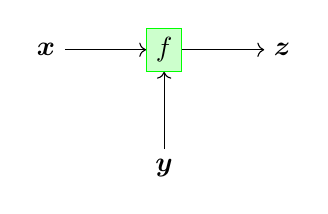
\begin{tikzpicture}
        \vnode (x) at (0,0) {$\inp$}; %
        \vnode (y) at (1.5,-1.5) {$\outp$}; %
        \vnode (z) at (3,0) {$\seq{z}$}; 
        \funnode (f) at (1.5,0) {$f$}; \draw[->] (x) -- (f); 
        \draw[->] (y) -- (f); 
        \draw[->] (f)  -- (z);
      \end{tikzpicture}
    \end{center}
    This node implements: 
    $$ \seq{z} = f(\inp,\outp)$$
  \end{block}

\end{frame}

\begin{frame}{A function node - 2}
  \begin{block}{Backward pass}
    \begin{columns}
    \begin{column}{0.4\textwidth}
    \begin{center}
      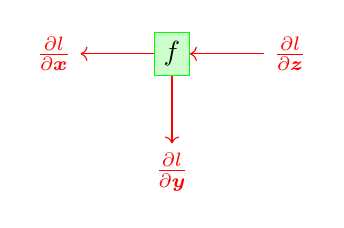
\begin{tikzpicture}
        \vnode[red] (x) at (0,0) {$\frac{\partial\ploss}{\partial\inp}$}; %
        \vnode[red] (y) at (1.5,-1.5) {$\frac{\partial\ploss}{\partial\outp}$}; %
        \vnode[red] (z) at (3,0) {$\frac{\partial\ploss}{\partial\seq{z}}$}; 
        \funnode (f) at (1.5,0) {$f$}; 
        \draw[->,red] (f) -- (x); 
        \draw[->,red] (f) -- (y); 
        \draw[->,red] (z)  -- (f);
      \end{tikzpicture} 
    \end{center}
    \end{column}
    \begin{column}{0.6\textwidth}
      A function node knows : 
      \begin{itemize}
      \item the  "local gradients'' computation
        $$\color{green} \frac{\partial\seq{z}}{\partial{\inp}}, \frac{\partial\seq{z}}{\partial{\outp}}$$
      \item how to return the gradient  to the inputs: 
        $$\big( {\color{red} \frac{\partial\ploss}{\partial\seq{z}}  }
        {\color{green} \frac{\partial\seq{z}}{\partial{\inp}}}\big), 
        \big( {\color{red} \frac{\partial\ploss}{\partial\seq{z}} }
        {\color{green} \frac{\partial\seq{z}}{\partial{\outp}}}\big)$$
      \end{itemize}
    \end{column}
    \end{columns}
  \end{block}  
\end{frame}


\begin{frame}{Summary of a function node}
  \begin{center}
    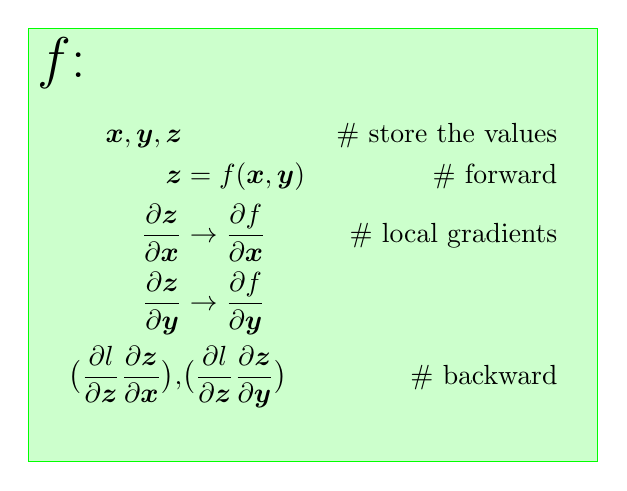
\begin{tikzpicture}
      \draw node[draw=green,fill=green!20,left,text width=7cm] {
        {\huge $f$:}
        \begin{align*}
          \inp,\outp,\seq{z}&  &\textrm{\# store the values}\\
          \seq{z} &= f(\inp,\outp)  &\textrm{\# forward}\\
           \frac{\partial\seq{z}}{\partial{\inp}} &\rightarrow \frac{\partial f}{\partial{\inp}}&\textrm{\# local gradients} \\
           \frac{\partial\seq{z}}{\partial{\outp}} &\rightarrow \frac{\partial f}{\partial{\outp}} \\
           \big(\frac{\partial\ploss}{\partial\seq{z}}\frac{\partial\seq{z}}{\partial{\inp}}\big), &\big(\frac{\partial\ploss}{\partial\seq{z}}\frac{\partial\seq{z}}{\partial{\outp}}\big)&\textrm{\# backward}\\
        \end{align*}
      };
    \end{tikzpicture}
  \end{center}
\end{frame}

\begin{frame}{Example of a single layer network}
            \begin{center}
          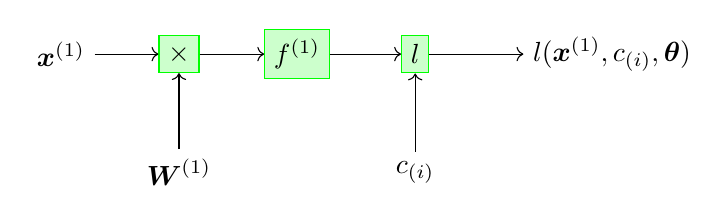
\begin{tikzpicture}
          \vnode (x2) at (0,0) {$\x\lid{1}$}; % 
          \vnode (W2) at  (1.5,-1.5) {$\W\lid{1}$};  % 
          \funnode (dot2) at (1.5,0) {$\times$};%
          \funnode (f2) at (3,0) {$f\lid{1}$}; 
          \funnode (loss) at (4.5,0) {$\ploss$}; 
          \vnode (label) at  (4.5,-1.5) {$\classi$};  % 
          \vnode (outloss) at  (7,0) {$\ploss(\x\lid{1},\classi,\params)$};  % 
          \draw[->] (x2) -- (dot2); 
          \draw[->] (dot2) -- (f2); 
          \draw[->] (W2) -- (dot2); 
          \draw[->] (f2) -- (loss);
          \draw[->] (label) -- (loss);
          \draw[->] (loss) -- (outloss);
        \end{tikzpicture}
        \end{center}
        \only<1>{
          \begin{block}{Forward}
            For each function node in topological order
              \begin{itemize}
              \item forward propagation
              \end{itemize}
              Which means:
              \begin{enumerate}
              \item $\seq{a}\lid{1} = \W\lid{1} \inp\lid{1}$
              \item $\outp\lid{1} = f\lid{1}(\seq{a}\lid{1})$
              \item $\ploss(\outp\lid{1},\classi)$
              \end{enumerate}
          \end{block}
        }
        \only<2>{
          \begin{block}{Backward} 
            For each function node in reversed topological order
              \begin{itemize}
              \item backward propagation
              \end{itemize}
              Which means:
              \begin{enumerate}
              \item $\pgrad{\outp\lid{1}}$
              \item $\pgrad{\seq{a}\lid{1}}$
              \item $\pgrad{\W\lid{1}}$
              \end{enumerate}
          \end{block}
        }
\end{frame}

\begin{frame}{Example of a two layers network}
  \begin{center}
    \input{../figs/mlp_computation_2}
  \end{center}
  \begin{itemize}
  \item The algorithms remain the same,
  \item even for more complex
    architectures
  \item Generalization by coding your own  function node or by
  \item Wrapping a layer in a module
  \end{itemize}
\end{frame}



%%%%%%%%%%%%%%%%%%%%%%%%%%%%%%%%%%%%%%%%%%%%%%%%%%%%%%%%%%%%%%%%%%%%%%
\section{Pytorch: Neural Network}
\begin{frame}{pytorch in three concepts}
  \begin{block}{A \textit{Tensor} is a tensor}
    \begin{itemize}
    \item Similar to numpy’s \textit{ndarrays}, but can be used on a
      GPU to accelerate computing.
    \item A node of a computation graph, holding:
      \begin{itemize}
      \item the gradient w.r.t to it self (back-propagation)
      \item a reference  to its creator
      \end{itemize}
    \end{itemize}
  \end{block}


  \begin{block}{\textit{Autograd}}
    Package for building computational graphs out of Tensors, and
    automatically computing gradients
  \end{block}
  
  \begin{block}{Module}
    A neural network layer,  may store state or
    learnable  Function (i.e with parameters)
  \end{block}
\end{frame}



\begin{frame}[fragile]{An example in pytorch}
  
  \begin{minted}{python}
    import torch as th
    # The model 
    D_in=2  # input size : 2 
    D_out=1 # output size: one value 
    model = th.nn.Sequential(
       th.nn.Linear(D_in, D_out),
       th.nn.Sigmoid()    
       )
    loss_fn = th.nn.BCELoss()
    # Optimizer will update  the weights of the model. 
    lr0 = 1e-4 
    optimizer = torch.optim.SGD(model.parameters(),
                       lr=lr0) 
  \end{minted}
\end{frame}

\begin{frame}[fragile]{An example in pytorch - 2}
  \begin{minted}{python}
    for t in  range(10): 
       # Forward pass: compute predicted y by passing x.  
       y_pred = model(x)
       # Compute and print loss.  
       loss = loss_fn(y_pred, y) 
       print(t, loss.data[0])
       # Optim in two steps
       optimizer.zero_grad()
       # Backward pass: compute gradient of the loss wrt parameters 
       loss.backward()
       # Calling the step function on an Optimizer makes an update 
       optimizer.step()
  \end{minted}
\end{frame}


\begin{frame}{Three kinds of \textit{Module}}

  
  \begin{block}{Linear}
    \begin{itemize}
    \item \textit{Linear} is a \textit{Module} for a linear
      transformation.
    \item The parameters: a \textit{Tensor} $\W$
    \item Forward $\x\rightarrow \W\x$
    \end{itemize}
  \end{block}


  \begin{block}{Sigmoid}
    \begin{itemize}
    \item \textit{Sigmoid} is a \textit{Module} for a pointwise function
    \item No parameters
    \end{itemize}
  \end{block}

  \begin{block}{Sequential}
    \begin{itemize}
    \item \textit{Sequential} is a container \textit{Module} 
    \item It contains a sequence of \textit{Module}, i.e a feed-forward NNet
    \end{itemize}
  \end{block}
  \begin{center}
    Look at the \textit{torch.nn} doc for many examples
  \end{center}
\end{frame}



\begin{frame}[fragile]{From CPU to GPU}
  \begin{minted}{python}
    # This vector is stored on cpu (+any operation you do on it)
    a = torch.DoubleTensor([1., 2.])
    # The same for GPU
    a = torch.FloatTensor([1., 2.]).cuda()
    a = torch.cuda.FloatTensor([1., 2.])
    # it will be on the default device: 
    torch.cuda.current_device()
    #####
    # For the model: 
    model = model.cuda()
  \end{minted}
\end{frame}

\begin{frame}[fragile]{Define your module}
  \begin{minted}{python}
    class LogisticRegression(th.nn.Module):
        def __init__(self,D_in):
           super(LogisticRegression, self).__init__()
           self.lin = th.nn.Linear(D_in, 1)
           self.out = th.nn.Sigmoid()    
    
        def forward(self, x): 
           a = self.lin(x)
           return self.out(a)
           
    mod = LogisticRegression(D_in=2)
  \end{minted}
\end{frame}











%%%%%%%%%%%%%%%%%%%%%%%%%%%%%%%%%%%%%%%%%%%%%%%%
\bibliographystyle{../styles/naaclhlt2012}
{\footnotesize \bibliography{./alex}}
%%%%%%%%%%%%%%%%%%%%%%%%%%%%%%%%%%%%%%%%%%%%%%%%
\end{document}
